%        File: slide.tex
%     Created: 三 7月 04 02:00 下午 2018 C
% Last Change: 三 7月 04 02:00 下午 2018 C
%
\documentclass{beamer}
\usepackage{graphicx}
\usepackage{xcolor}
\usepackage{ctex}
\usepackage{listings}
\usepackage{amsmath}
\usepackage{amssymb}
\usepackage{xeCJK}
\usepackage{xcolor}
\lstset{language = c,numbers=left,keywordstyle= \color{blue!70},commentstyle=\color{red!50!green!50!blue!50},frame=shadowbox,rulesepcolor= \color{red!20!green!20!blue!20}} 
\hypersetup{colorlinks,linkcolor = green, urlcolor = green}

\title{网络传输机制实验}
%\subtitle{}
\institute{University of Chinese Academy of Sciences}
\author{冯吕}
\date{\today}
%\usetheme{AnnArbor}
%\usetheme{Madrid}
%\usetheme{Montpellier}
%\usetheme{Szeged}
\usetheme{CambridgeUS}
%\usetheme{Berlin}
%\usetheme{Boadilla}
\usecolortheme{default}
%\usecolortheme{beaver}
%\usecolortheme{dolphin}
\begin{document}
\CJKfamily{zhsong}
\zihao{5}

\begin{frame}
  \titlepage
  \begin{figure}[ht]\centering
\includegraphics[scale=0.3]{./fig/ucas.jpg}\end{figure}
\end{frame}

\begin{frame}{主要内容}
  \tableofcontents
\end{frame}
 
\section{传输实验一:连接管理与socket实现}

\begin{frame}{建立连接}
  \begin{block}{}
  $TCP$传输机制中连接建立的关键在于三次握手.
\end{block}
\begin{itemize}
  \item 主动建立连接:
	\begin{itemize}
	  \item 发送目的端口的$SYN$数据包$\rightarrow TCP\_SYN\_SENT$ ($connect$);
		\item 收到$SYN\mid ACK$数据包 : 第二次握手;
		  \item 回复$ACK$数据包$\rightarrow TCP\_ESTABLISHED$;
	\end{itemize}
	\item 被动建立连接:
	  \begin{itemize}
		\item  申请占用一个端口号:$bind$;
		  \item 监听端口号:$listen$;
			\item 收到$SYN$数据包$\rightarrow TCP\_SYN\_RECV$ : 第一次握手;
			  \item 回复$SYN\mid ACK$数据包;
				\item 收到$ACK$数据包$\rightarrow TCP\_ESTABLISHED$ : 第三次握手;
	  \end{itemize}
\end{itemize}
\end{frame}

\begin{frame}[fragile]{主动建立连接}
  主动连接远程$tcp\ socket$:
  \begin{figure}[H]
	\centering
	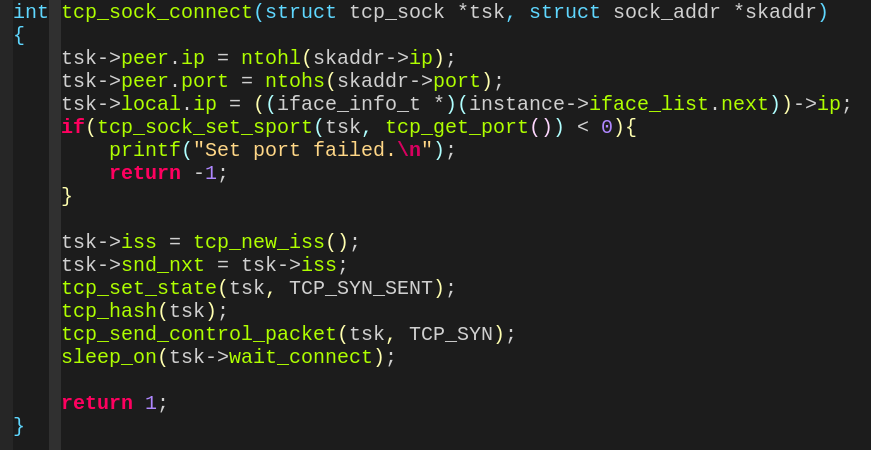
\includegraphics[scale = 0.35]{./fig/cnt.png}
  \end{figure}
\end{frame}

\begin{frame}{Listen}
{tcp\_sock\_listen}设置$backlog$,进入$TCP\_LISTEN$状态,同时将$tcp\ sock\ hash$到$listen\ table$上:
  \begin{figure}[H]
	\centering
	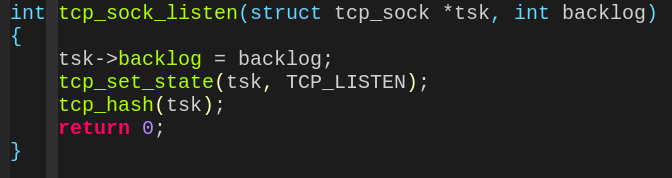
\includegraphics[scale = 0.4]{./fig/lst.png}
  \end{figure}
\end{frame}

\begin{frame}{被动建立连接}
{tcp\_sock\_accept} 如果$accept\ queue$不为空,弹出第一个$tcp\ sock$,否则,$sleep\ on\ wait\_accept$:
  \begin{figure}[H]
	\centering
	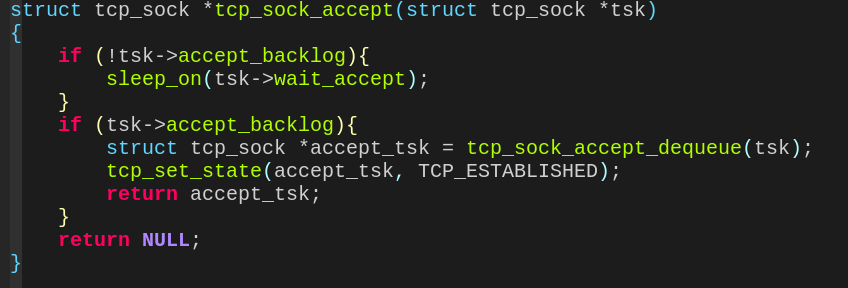
\includegraphics[scale = 0.35]{./fig/acp.png}
  \end{figure}
\end{frame}

\begin{frame}{Look Up}{tcp\_sock\_lookup\_established}
  对于一个新到达的数据包,需要先在$established\ table$中查找$socket$:
  \begin{figure}[H]
	\centering
	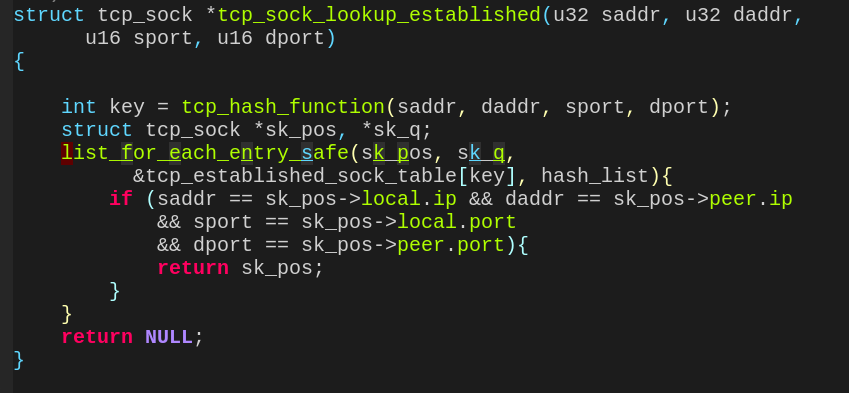
\includegraphics[scale = 0.35]{./fig/est.png}
  \end{figure}
\end{frame}

\begin{frame}{Look Up}{tcp\_sock\_lookup\_listen}
  如果在$established\ table$中没有找到对应的$socket$,再到$listen\ table$中查找:
  \begin{figure}[H]
	\centering
	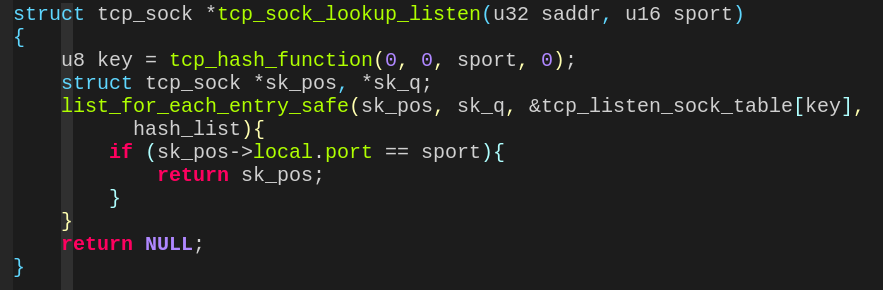
\includegraphics[scale = 0.35]{./fig/looklis.png}
  \end{figure}
\end{frame}

\begin{frame}{tcp\_state\_listen}
  被动连接的一方处于$TCP\_LISTEN$状态时收到包(第一次握手):
  \begin{figure}[H]
	\centering
	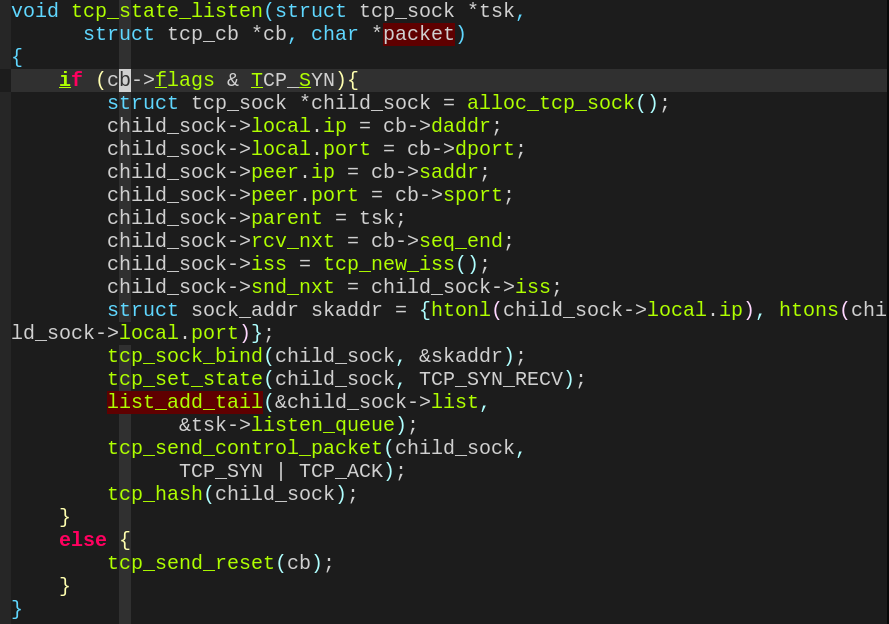
\includegraphics[scale = 0.32]{./fig/state_lis.png}
  \end{figure}
\end{frame}

\begin{frame}{tcp\_state\_syn\_sent}
  主动连接的一方处于$TCP\_SYN\_SENT$状态时收到包(第二次握手):
  \begin{figure}[H]
	\centering
	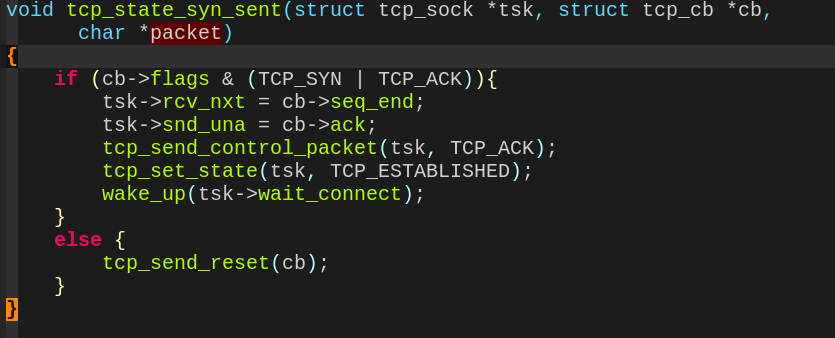
\includegraphics[scale = 0.35]{./fig/syn_sent.png}
  \end{figure}
\end{frame}

\begin{frame}{tcp\_state\_syn\_recv}
  被动连接的一方处于$TCP\_SYN\_RECV$状态时收到包(第三次握手):
  \begin{figure}[H]
	\centering
	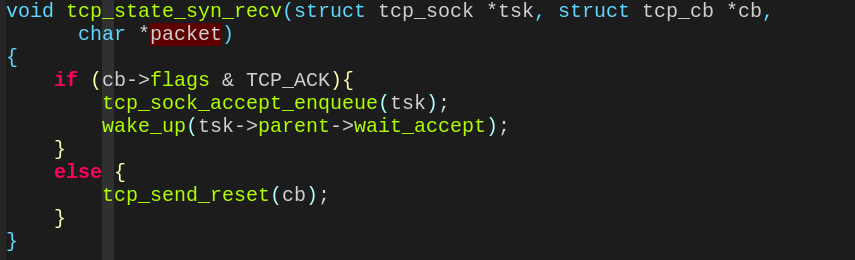
\includegraphics[scale = 0.35]{./fig/syn_recv.png}
  \end{figure}
\end{frame}

\begin{frame}{关闭连接}
  \begin{itemize}
	\item 主动关闭:
	  \begin{itemize}
		\item 发送$FIN$包,进入$TCP\_FIN\_WAIT\_1$状态;
		\item 收到$FIN$对应的$ACK$包,进入$TCP\_FIN\_WAIT\_2$状态;
		\item 收到对方发送的$FIN$包,回复$ACK$,进入$TCP\_TIME\_WAIT$状态;
		\item 等待$2*MSL$时间,进入$TCP\_CLOSED$状态,连接结束;
	  \end{itemize}
	  \item 被动关闭:
		\begin{itemize}
		  \item 收到$FIN$包,回复相应的$ACK$, 进入$TCP\_CLOSE\_WAIT$状态;
		  \item 当自己没有待发数据时,发送$FIN$包,进入$TCP\_LAST\_ACK$状态;
		  \item 收到$FIN$包对应的$ACK$,进入$TCP\_CLOSED$状态,连接结束;
		\end{itemize}
  \end{itemize}
\end{frame}

\begin{frame}{接收数据包处理流程}
  $tcp\_process$: 需要根据$socket$当前所处的状态和包的类型进行对应的处理:
  \begin{itemize}
	\item 检查TCP校验和是否正确;
	  \item 检查是否为RST包,如果是,直接结束连接;
		\item 检查是否为SYN包,如果是,进行建立连接管理;
		  \item 检查ack字段,对方是否确认了新的数据;
			\item 检查是否为FIN包,如果是,进行断开连接管理;
  \end{itemize}
\end{frame}

\section{传输实验二:数据收发}
\begin{frame}{无丢包情况下的数据收发}
  本次实验需要实现无丢包环境下的数据收发:
  \begin{itemize}
	\item $tcp\_sock\_write$封装数据包,然后将数据包从$IP$层发送出去, $socket$收到数据包后将数据写到接收缓存中,同时回复$ACK$;
	  \item $tcp\_sock\_read$从接收缓存中读取数据到上层应用$buff$中;
		\item 读写过程中需要使用锁来对缓存进行互斥访问:在$ring\_buffer$中添加一个锁;
  \end{itemize}
\end{frame}

\begin{frame}{tcp\_sock\_write}
  将上层应用$buff$中的数据封装成数据包发送出去,如果当前发送窗口为$0$,则$sleep\ on\ wait\_send$:
  \begin{figure}[H]
	\centering
	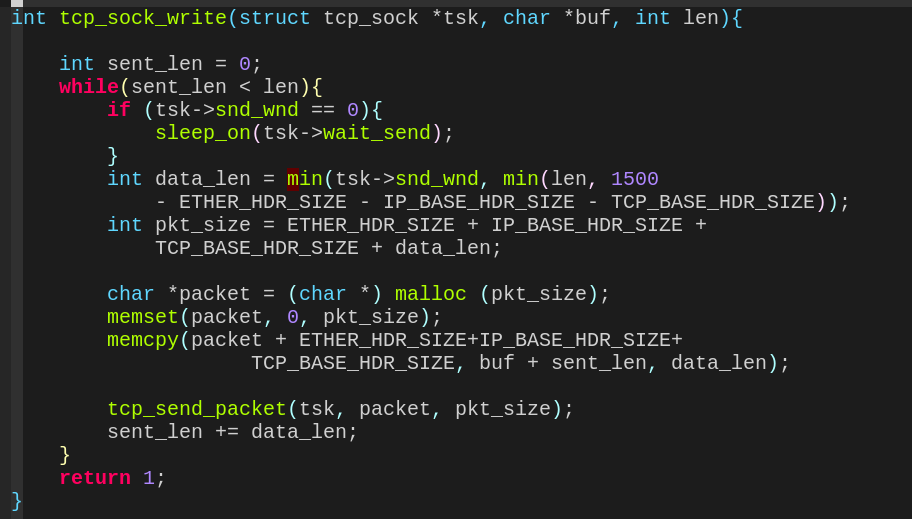
\includegraphics[scale = 0.35]{./fig/write.png}
  \end{figure}
\end{frame}

\begin{frame}{tcp\_sock\_read}
  从$socket$的接收缓存中读取数据,如果当前没有数据, 则$sleep\ on \ wait\_recv$:
  \begin{figure}[H]
	\centering
	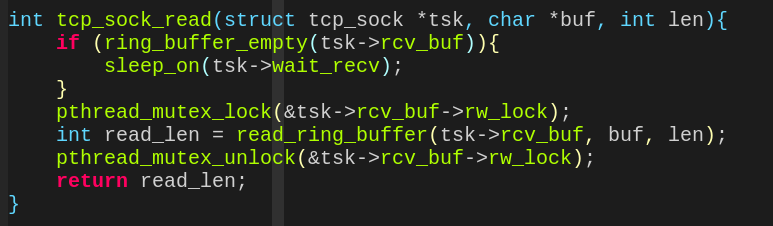
\includegraphics[scale = 0.35]{./fig/read.png}
  \end{figure}
\end{frame}

\begin{frame}{收到数据包的处理}
  \begin{itemize}
	\item 当收到包含数据的数据包时,将数据写入到$ring\_buffer$中,同时$wake\_up \ wait\_recv$, 然后回复$ACK$;
	  %\item 从$ring\ buffer$中读取数据之后,更新窗口;
	  \item 当收到$ACK$数据包时,$update\ sending\ window$;
  \end{itemize}
\end{frame}

\section{传输实验三:可靠传输}

\begin{frame}[fragile]{可靠传输}
  \begin{itemize}
	\item 
  实验三需要实现在丢包环境下的可靠传输。
  \item 在$tcp\_sock$中增加三个成员:
\begin{lstlisting}
struct tcp_timer retrans_timer; // 超时重传
//定时器
struct list_head send_buf;//未确认数据
struct list_head rcv_ofo_buf;//不连续数据
//存于send_buf/ofo_buf中的数据结构
struct send_packet{
    struct list_head list;
    char *packet;
    int len;
};
struct ofo_packet{
    struct list_head list;
    char *packet;
    int len;
    int seq_num;
};
\end{lstlisting}
  \end{itemize}
\end{frame}

\begin{frame}[fragile]{修改$send\ packet$}
  \begin{itemize}
	\item 修改$tcp\_send\_packet$:当发送一个$packet$时,将其存到$send\_buf$中,同时启动一个重传定时器;
\begin{lstlisting}
struct send_packet *send_pkt = (struct 
send_packet *)malloc(sizeof(struct send_packet));
send_pkt->packet = (char *)malloc(len);
send_pkt->len = len;
memcpy(send_pkt->packet, packet, len);
list_add_tail(&send_pkt->list, &tsk->send_buf);
tcp_set_retrans_timer(tsk);
\end{lstlisting}
\item 修改$tcp\_send\_control\_packet$ : 如果发送的是$SYN\mid FIN$包,也需要将其存到$send\_buf$中,直到收到$ACK$;
  \end{itemize}
\end{frame}

\begin{frame}{tcp\_timer}
  \begin{itemize}
	\item 在$tcp\_timer$中增加一项:重传次数;
	  \item 设置重传定时器和关闭定时器:
		\begin{figure}[H]
		  \centering
		  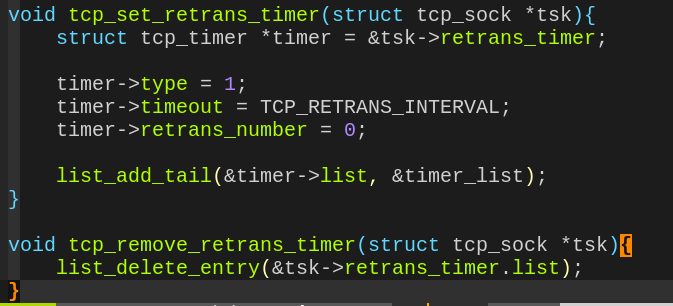
\includegraphics[scale = 0.35]{./fig/try_timer.png}
		\end{figure}
  \end{itemize}
\end{frame}

\begin{frame}{修改$tcp\_scan\_timer\_list$}
  \begin{itemize}
	\item (1)判断定时器类型,如果类型为$wait$,则根据是否$timeout$关闭即可,如果类型为$retrans$,转(2);
	\item (2)判断重传次数是否小于$3$,如果不小于,则关闭该$timer$对应的$socket$,否则转(3);
	\item (3)重传$send\_buf$中的包,更新定时器:$timeout*2, retrans\_number + 1$
  \end{itemize}
\end{frame}

\begin{frame}{收到$ACK$}
  当收到$ACK$时,将$send\_buf$中$sep\_end <ack$的包移除,同时更新定时器:
  \begin{figure}[H]
	\centering
	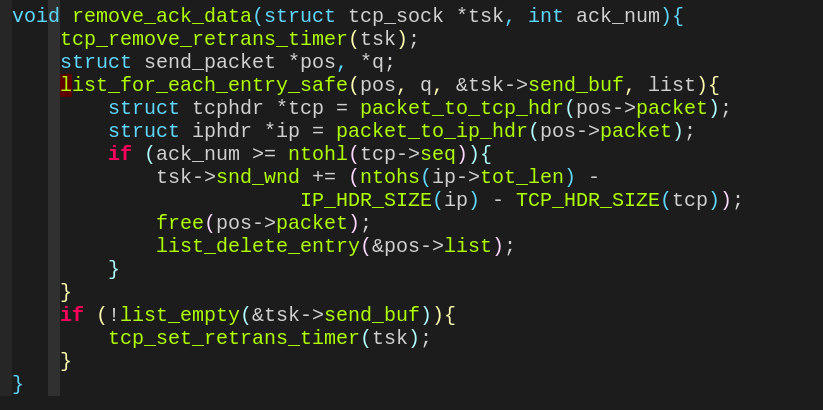
\includegraphics[scale = 0.35]{./fig/rmv_ack.png}
  \end{figure}
\end{frame}

\begin{frame}{收到连续数据}
  如果收到连续的数据:$cb->seq  = = tsk->rcv\_nxt$
  \begin{itemize}
	\item $(1)$将数据写到$ring\_buffer$中:$write\_ring\_buffer()$
	\item $(2) tsk->rcv\_nxt = cb->seq\_end$,并$wake\_up\ wait\_recv$
	\item $(3)$判断$ofo\ buffer$中是否出现连续数据($packet->seq = = tsk->rcv\_nxt$),则将数据从$ofo\ buffer$中写到$ring\ buffer$中。
  \end{itemize}
\end{frame}

\begin{frame}[fragile]{收到不连续数据}
  如果收到不连续数据:$cb->seq > tsk->rcv\_nxt$,则将数据包存到$ofo\_buffer$中:
\begin{lstlisting}
struct ofo_packet *buf_pac = (struct ofo_packet *)
     malloc(sizeof(struct ofo_packet));
buf_pac->packet = (char *)malloc(cb->pl_len);
buf_pac->len = cb->pl_len;
buf_pac->seq_num = cb->seq;
memcpy(buf_pac->packet, cb->payload, cb->pl_len);
list_add_tail(&buf_pac->list, tsk->rcv_ofo_buf);
\end{lstlisting}
\end{frame}

\begin{frame}
  \begin{center}
  %\begin{block}{}
	\zihao{0}
	\CJKfamily{zhkai}
	谢谢!
  %\endblock}
\end{center}
\end{frame}
\end{document}


